\section{Data Lake}
In der Einleitung (\cref{sec:einleitung-datalake}) wurde der Data Lake als Lösung für die Probleme der Datenerfassung im Big-Data-Bereich bereits kurz beschrieben.
In diesem Abschnitt wird noch einmal genauer auf Data-Lake-Systeme, deren Definition, Architektur und existierende Systeme eingegangen.

\subsection{Definition eines Data Lake}
Neben der Definition, die in der Einleitung gegeben wird, wurde von \textcite{sawadogo2021data} eine detailliertere Definition für Data Lakes aufgestellt.
Hiernach sind Data-Lake-Systeme ein skalierbarer Speicher für Daten jeden Typs.
Die Daten werden im Rohformat gespeichert und hauptsächlich durch Datenspezialisten, wie Statistiker oder Analysten, für die Extraktion von Wissen verwendet.
Ein Data Lake hat dabei die folgenden Eigenschaften: \begin{enumerate}
    \item ein Metadaten-Katalog, um die Datenqualität sicher zu stellen,
    \item Regeln und Werkzeuge für die Data Governance,
    \item Zugänglichkeit zu den Daten für verschiedene Arten von Benutzern,
    \item die Integration von Daten jeden Typs,
    \item sowohl eine logische als auch eine physische Gliederung und
    \item die Skalierbarkeit von Speicher und Verarbeitung.
\end{enumerate}

\subsection{Architekturen für Data Lakes}
Von \textcite{inmon2016data} wird das System in sogenannten Ponds (Teiche) strukturiert.
Jeder Pond ist mit einem spezialisierten Speichersystem verknüpft und beinhaltet Daten eines bestimmten Typs.
Einige Ponds führen zudem weitere Verarbeitungen der Daten, wie Aufbereitung oder Analysen aus.
Inmon hat eine Architektur aus fünf Ponds aufgestellt (\cref{fig:datalake-ponds}).
\begin{enumerate}
    \item Daten werden im \emph{Raw Data Pond} im Rohformat gespeichert und fließen von dort aus in andere Ponds.
          Dieser dient also als Eintrittspunkt in das System für neue Daten.
          Nach dem Verlassen des Pond werden die Daten aus diesem gelöscht.
    \item Der \emph{Analog Data Pond} enthält analoge Daten, meist von IoT-Geräten.
          Diese werden hier auf ein aussagekräftiges und verwaltbares Volumen reduziert und umstrukturiert.
    \item In den \emph{Application Data Pond} kommen Daten, die von Software-Anwendungen erzeugt wurden.
          Diese sind häufig strukturierte Daten aus relationalen Daten\-bank-Systemen.
          Sie werden für Analysen integriert und aufbereitet.
    \item Der \emph{Textual Data Pond} enthält unstrukturierte Daten und Prozesse, die deren Analyse erleichtern.
    \item Im \emph{Archival Data Pond} werden alle Daten gespeichert, die nicht mehr aktiv verwendet, aber eventuell in der Zukunft nochmal gebraucht werden.
\end{enumerate}
\begin{figure}
    \centering
    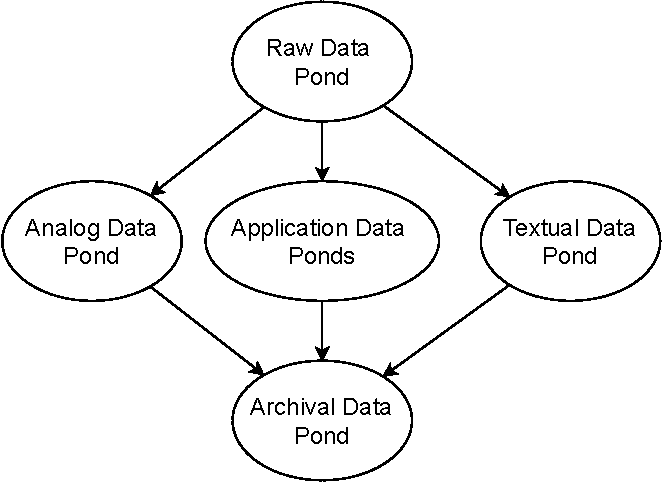
\includegraphics[width=.8\textwidth]{Grafiken/Grundlagen-Ponds.pdf}
    \caption{Ponds-Architektur \parencite[nach: ][S. 27]{inmon2016data}}
    \label{fig:datalake-ponds}
\end{figure}

Ein anderer Ansatz ist die Unterteilung des Data Lake in Zonen (\cref{fig:datalake-zones}).
Hier werden die Daten nach ihrem Verfeinerungsgrad in einer entsprechenden Zone abgelegt.
Dabei durchlaufen sie die einzelnen Zonen hintereinander.
Die Anzahl der Zonen und deren Verfeinerungsgrad ist dabei je nach Anwendung unterschiedlich \parencite{dl-zones}.

\begin{figure}
    \centering
    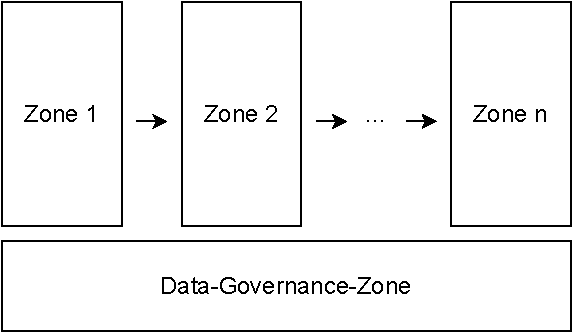
\includegraphics[width=.8\textwidth]{Grafiken/Grundlagen-Zones.pdf}
    \caption{Prinzip der Zonen-Architektur}
    \label{fig:datalake-zones}
\end{figure}

Eine speziellere Architektur ist die Lambda-Architektur, die für die verteilte Verarbeitung von Echtzeit- und Batch-Daten verwendet wird.
Eine Lambda-Architektur besteht aus drei Ebenen (Layers) \parencite{lambda-arch}: \begin{enumerate}
    \item Die \emph{Batch Layer} hat zwei Aufgaben.
          Die erste Aufgabe ist das verteilte Speichern von wachsenden Daten.
          Dafür kann zum Beispiel das HDFS verwendet werden.
          Als zweite Aufgabe werden Batch Views für die verteilten Daten vorberechnet, um Anfragen schneller beantworten zu können.
    \item In der \emph{Speed Layer} werden inkrementell Echtzeit-Views auf Daten verwaltet.
          Dadurch wird die Lücke gefüllt, die bei den Views in der Batch-Ebene entstehen können.
          Die Speed Layer enthält immer nur aktuelle Daten.
          Ältere Daten werden durch die Batch Layer aufgenommen.
    \item Die \emph{Serving Layer} enthält Indices über alle Batch Views um Anfragen mit geringer Latenz bearbeiten zu können. Sie ist dafür verantwortlich die Views aus der Batch und der Speed Layer zusammenzuführen um Echtzeitergebnisse über alle Daten bereit zu stellen.
\end{enumerate}

Nach \textcite{sawadogo2021data} können die Architekturen von Data-Lake-Systemen auch anders unterteilt werden.
Bei datenorientierten Architekturen wird der Data Lake in verschiedene Datenbereiche unterteilt.
Die funktionsorientierten Architekturen dagegen teilen das Data-Lake-System nach den Funktionen auf, die in ähnlichen Bereichen zusammengefasst werden.
Ein Beispiel ist die Architektur aus der Einleitung von \textcite{datalake_03}.
In hybriden Architekturen können auch beide Ansätze kombiniert werden.

\subsection{Data-Lake-Systeme und Rahmenwerke}
Es gibt bereits verschiedene Rahmenwerke oder Systeme für die Umsetzung eines Data Lake.
Nachfolgend wird eine Auswahl daraus vorgestellt.

\paragraph{CoreDB} CoreDB ist ein Service, der es erlaubt über eine einzige REST-API Daten und Metadaten in einem Data Lake zu organisieren, zu indizieren und abzufragen.
Es können sowohl relationale als auch NoSQL-Datenbanksysteme mit CoreDB verwendet werden.
Für die Suche in den Daten wird elastic\footnote{https://www.elastic.co/} verwendet.
Das Design von CoreDB unterstützt Funktionen für die Sicherheit und Zugriffskontrolle und die Verfolgung und Herkunft, um überwachende Metadaten sammeln zu können \parencite{coredb}.

\paragraph{Azure Data Lake} In dem Cloud-Angebot von Microsoft gibt es den Azure Data Lake\footnote{https://azure.microsoft.com/de-de/solutions/data-lake/}.
Hier werden viele Funktionen, die für den Aufbau eines Data Lake notwendig sind als Cloud-Lösung bereitgestellt.
Dazu gehören unter anderem Hadoop, Apache Spark und ein Speichersystem zum Speichern aller Daten.
Außerdem gibt es weitere Dienste zur Analyse oder Integration der Daten.

\paragraph{Kylo} Kylo\footnote{https://kylo.io/} ist ein Projekt für eine Data-Lake-Management-Plattform.
In dieser Plattform ist eine Ingestion-Komponente enthalten, die die Bereinigung und Validierung von Daten unterstützt.
Außerdem gibt es Funktionen für die Aufbereitung und Erkundung von Daten oder zur Systemüberwachung.
Zusätzlich ist Apache Nifi\footnote{https://nifi.apache.org/} zur Erstellung von Verarbeitungs-Pipelines integriert.
Die Entwicklung an Kylo wird seit über einem Jahr nicht mehr fortgeführt.

\paragraph{Hudi} Apache Hudi\footnote{https://hudi.apache.org/} ist eine Plattform, um selbst-verwaltete Data Lakes mit einer Optimierung für Datenstromverarbeitung aufzubauen.
Zu den Features von Hudi gehört zum Beispiel die Indizierung von Änderung und das Zurückgehen in den Daten zu einem bestimmten Zeitpunkt.
Hudi unterstützt sowohl inkrementelle Abfragen als auch Batch-Verarbeitung von Daten.

\paragraph{}
Bei diesen Systemen fehlen entweder eine ausführliche Metadatenpflege oder eine Datenversionierung, sie bilden nur einen bestimmten Teil eines Data Lake oder sind für spezielle Anwendungsfälle.
Daher wurde bisher kein geeignetes Data-Lake-System für die Anwendung am HIT gefunden

\subsection{Delta Lake}

Als eine Lösung für die Versionierung von Daten gibt es den Delta Lake
Delta Lake ist eine extra Speicherebene, die auf dem HDFS oder eine Objektspeicher in der Cloud, wie Amazons S3, angewendet werden kann.
Das Ziel ist es, diesen Speichern ACID-Transaktionen, schnelles Arbeiten mit Metadaten der Tabelle und eine Versionierung der Daten hinzuzufügen.
Daten werden in sogenannten Delta-Tabellen mit Metadaten und Logs gespeichert.

Eine Delta-Tabelle wird zunächst durch ein Verzeichnis im Dateisystem dargestellt.
Die tatsächlichen Daten werden in diesem Verzeichnis als Parquet-Dateien abgelegt.
Dabei können die Daten auch noch in Unterverzeichnisse aufgeteilt werden, zum Beispiel für jedes Datum ein Verzeichnis.
Neben den Datenverzeichnissen gibt es in jeder Delta-Tabelle einen Ordner für die Logs in Form von JSON Dateien mit aufsteigender Nummerierung.
Metadaten werden sowohl innerhalb der Parquet- als auch in der Log-Dateien gespeichert.

Im Delta Lake wird ein Protokoll für den Zugriff verwendet, dass es mehreren Clients ermöglicht gleichzeitig Lesen zu können, aber immer nur einem das Schreiben erlaubt.
Dabei werden beim Schreiben immer erst neue Datensätze, die zur Tabelle hinzugefügt werden sollen, in das Verzeichnis der Delta-Tabelle geschrieben.
Danach wird eine neu Log-Datei erstellt.

Beim Lesen werden die Log-Dateien als Grundlage verwendet um daraus zusammen mit den gespeicherten Daten den Zustand der Tabelle an einem bestimmten Zeitpunkt zu erzeugen.
Standardmäßig wird beim Lesen immer die aktuellste Version verwendet, man kann aber auch eine bestimmte Version angeben.
Um den Aufwand bei der Verarbeitung der Logs zu verringern wird periodisch ein Kontrollpunkt erzeugt, bei dem alle vorherigen Logs zusammengefügt und komprimiert werden.
Das bedeutet, dass zum Beispiel das Operationen die sich gegenseitig aufheben nicht gespeichert werden.
Damit reicht es aus nur den letzten Checkpoint vor der zu lesenden Version und alle darauf folgende Logs zu lesen.

Durch das Design werden keine eigenen Server für die Pflege der Delta-Tabellen benötigt.
Diese Funktionen werden von den Clients übernommen.
Der Delta Lake unterstützt sowohl die Batch-Verarbeitung von Daten als auch Datenströme und bietet volle Integration in Spark \parencite{deltalake}.


\subsection{Existierender Data-Lake-Prototyp}
In einem Masterprojekt an der Hochschule Niederrhein \parencite{prototyp} wurde ein Prototyp für ein Data-Lake-System entwickelt.
In \cref{fig:prototyp-architektur} ist ein Überblick über dessen Architektur zu sehen.
Es handelt sich hierbei um eine Client-Server-Anwendung.
Der Client besteht aus einer Web-Anwendung über die Benutzer mit dem Data-Lake-System interagieren.
Er kommuniziert mit dem Server über eine REST-API, die auch durch andere Clients verwendet werden könnte.
Die Datenverarbeitung wird über ein Spark-Cluster gelöst.
Zum Speichern der Daten stehen drei verschiedene System zu Verfügung.
Es kommen eine PostgreSQL Datenbank für strukturierte, eine MongoDB für semistrukturierte und ein HDFS für unstrukturierte Daten zum Einsatz.

\begin{figure}
    \centering
    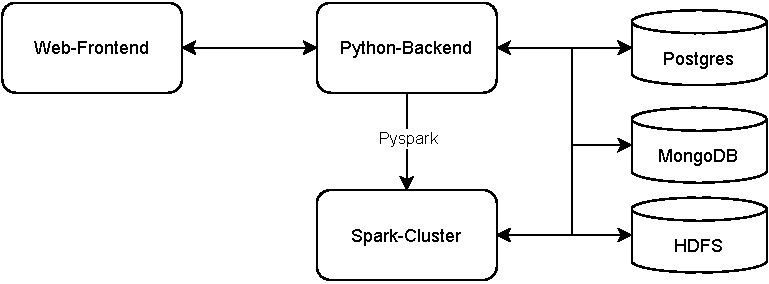
\includegraphics{Grafiken/Prototyp-Architektur.pdf}
    \caption[Architektur des Prototyp]{Architektur des Prototyp}
    \label{fig:prototyp-architektur}
\end{figure}

Die Verarbeitung der Ingestion ist im Prototyp abhängig von der Datenquelle und dem ausgewählten Zielspeicher.
In \cref{fig:prototyp-ingestion}  sind die verschiedenen Wege zu sehen.
Diese Verarbeitungsweise hat zwei Probleme, die in der neuen Ingestion gelöst werden müssen.
Dadurch, dass der Benutzer aus den verschiedenen Speichern ein Ziel auswählt, können hier leicht Probleme entstehen, falls die Datenquelle nicht mit dem Format des Speichers kompatibel ist.
Außerdem sind die Verarbeitungen der Quellen zu den Speichern fest im Code des Servers einprogrammiert.
So ist es nicht möglich während der Laufzeit neue Datenquellen zu integrieren.

\begin{figure}
    \centering
    \subfigure[Datenbank-Ingestion]{
        \label{fig:prototyp-db-ingeston}
        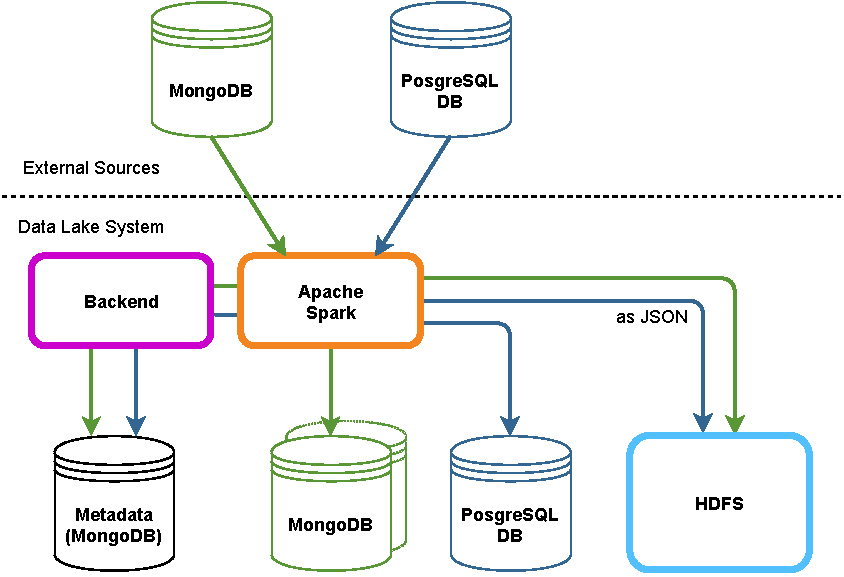
\includegraphics[width=.45\textwidth]{Grafiken/db_ingestion.pdf}
    }
    \subfigure[Datei-Ingestion]{
        \label{fig:prototyp-file-ingeston}
        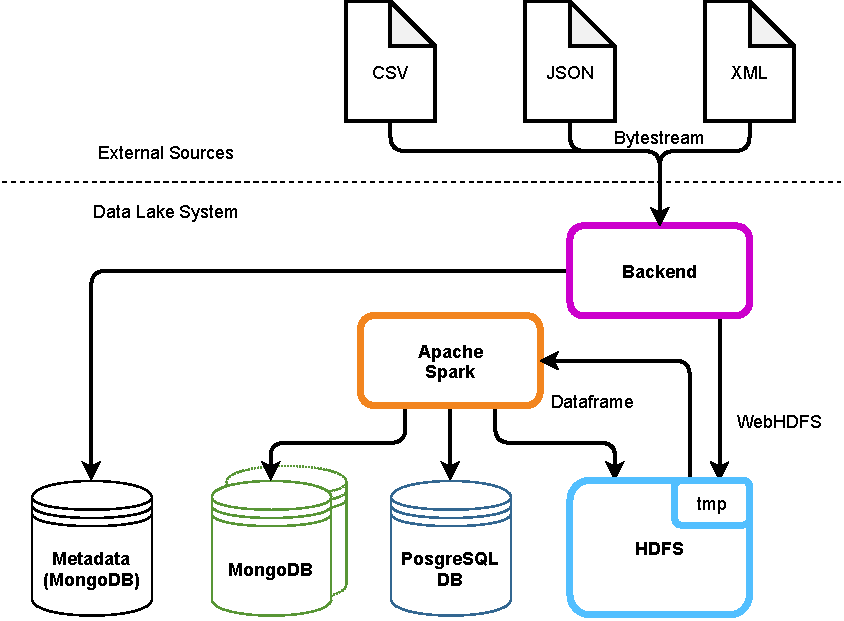
\includegraphics[width=.45\textwidth]{Grafiken/file_ingestion.pdf}
    }
    \caption[Ingestion-Verarbeitung des Prototyp]{Ingestion-Verarbeitung des Prototyp, \textcite[Quelle:][S. 3]{prototyp}}
    \label{fig:prototyp-ingestion}
\end{figure}

Im Vorlauf dieser Arbeit wurde ein Refactoring des Prototyp durchgeführt.
Dabei wurde festgestellt, dass die Erweiterung des Data-Lake-Systems um die Kompatibilität mit weiteren Datenquellen ein aufwändiger Prozess ist.
Auch durch die gewählten Speichersysteme für die geladenen Daten erschweren die Integration einer Lösung für die Versionierung der Daten.
Daher wurde beschlossen, dass eine dedizierte Ingestion-Schnittstelle für das System entwickelt werden soll.